\section{实验与结果}
\frame
{
  \frametitle{\secname~ }
  \begin{block}{数据集}
  \end{block}
  \begin{block}{准确率度量方式}
  \end{block}
  \begin{block}{VOC 2012实验结果}
  \end{block}
  \begin{block}{SIFT FLOW实验结果}
  \end{block}
}
\subsection*{数据集与度量方式}
\frame{
	\frametitle{Pascal VOC 2012 \& SIFT FLOW数据集}
   \vspace{-0.8em}
	\begin{figure}
		\centering
		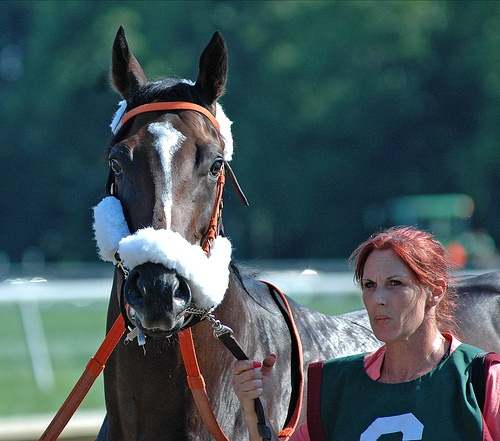
\includegraphics[width=.25\textwidth,height=.15\textwidth]{image/example/2007_000799.jpg}
		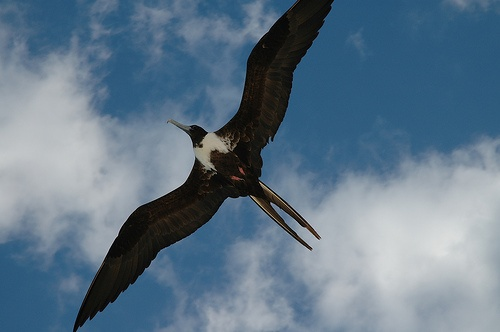
\includegraphics[width=.25\textwidth,height=.15\textwidth]{image/example/2007_002094.jpg}
		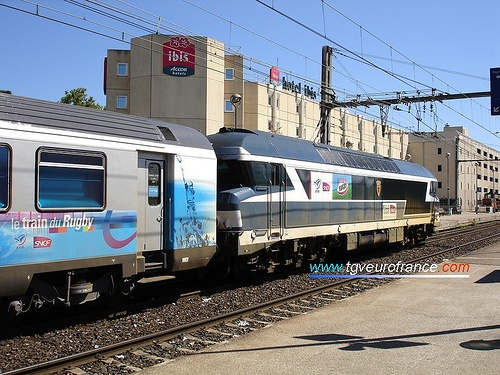
\includegraphics[width=.25\textwidth,height=.15\textwidth]{image/example/2007_004483.jpg}
		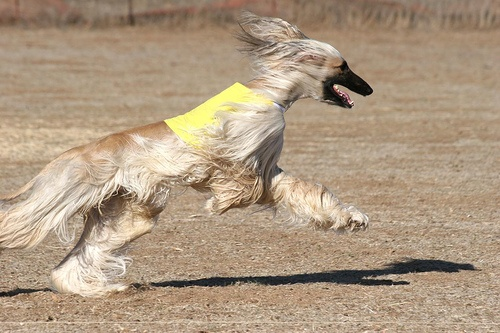
\includegraphics[width=.25\textwidth,height=.15\textwidth]{image/example/2007_003194.jpg}
		\caption{VOC 2012数据集:10582 张训练样本,1464张验证样本和1456张测试样本,21个类别}
	\end{figure}	
   \vspace{-1.8em}
	\begin{figure}[h]
		\centering
		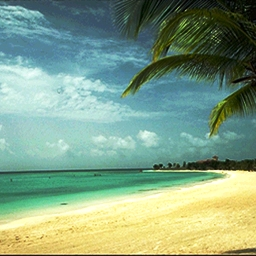
\includegraphics[width=0.25\textwidth,height=.15\textwidth]{figures/siftflow/coast_bea10.jpg}
		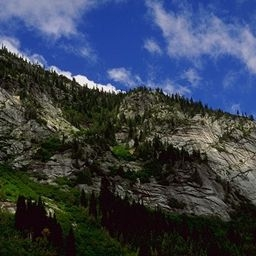
\includegraphics[width=0.25\textwidth,height=.15\textwidth]{figures/siftflow/mountain_n18058.jpg}
		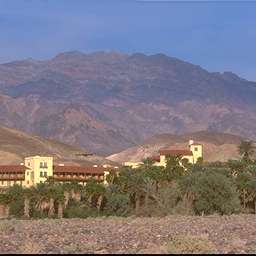
\includegraphics[width=0.25\textwidth,height=.15\textwidth]{figures/siftflow/opencountry_land732.jpg}
		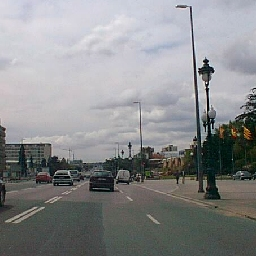
\includegraphics[width=0.25\textwidth,height=.15\textwidth]{figures/siftflow/highway_gre644.jpg}
		\caption{SIFT FLOW数据集:2488张训练样本,200张测试样本,33个类别}
		\label{fig:crop}
	\end{figure}
	\vspace{-1.2em}
	\footnotesize
	\begin{block}{图像预处理}
	\vspace{-0.5em}
	\begin{itemize}
		\item 训练时图像均缩放为321*321
		\item 随机选取训练图像,随机取镜像,数据白化
	\end{itemize}
	\end{block}
}

\frame{
   \frametitle{准确率度量方式}
   \begin{block}{}
设$n_{ij}$为真实值属于类别$i$但被分类为类别$j$的像素个数,$n_{cl}$表示有多少种不同的标签,$t_i=\sum_{j=1}^{n_{cl}}n_{ij}$为所有真实值为类别$i$的像素个数。
	\begin{align}
		\begin{split}
		\mbox{像素准确率} &= \sum_{i=1}^{n_{cl}}n_{ii} / \sum_{i=1}^{n_{cl}}t_i \\
			\mbox{平均像素准确率} &= \frac{1}{n_{cl}} \sum_{i=1}^{n_{cl}}(n_{ii}/ t_i) \\
		\mbox{Mean IU} &= \frac{1}{n_{cl}} \sum_{i=1}^{n_{cl}}\frac{n_{ii}}{t_i + \sum_j^{n_{cl}} n_{ji} - n_{ii}}
		\end{split}
	\end{align}
\end{block}
}
\subsection*{VOC 2012结果}
\frame{
   \frametitle{网格型长短记忆网络层数的选择}
   \begin{columns}
	   \begin{column}{0.5\textwidth}
			\vspace{-0.8em}
			\begin{figure}
				\centering
				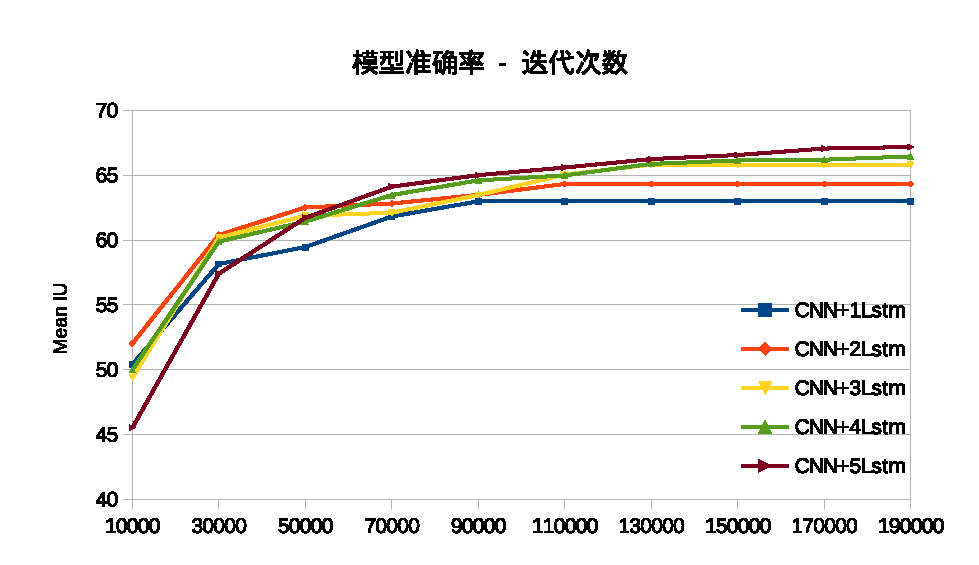
\includegraphics[width=\textwidth]{image/result/combine.eps}
				\caption{网格型长短记忆层数的不同对网络分割效果的影响方法}
				\label{fig:trainingaccuracy}
			\end{figure}
		\end{column}
	\vspace{-1.1em}
	\begin{column}{0.5\textwidth}
			\footnotesize
			\begin{itemize}
				\item[\dag] 在一定范围内增加长短记忆层数可以有效提高网络效果
				\item[\dag] 增加了5层网格型长短记忆网络之后,网络效果提升了\textbf{7.5\%}
			\end{itemize}
		\end{column}
	\end{columns}
	\vspace{-1em}
	\begin{figure}[h]
	\centering
		\makebox[0.11\textwidth]{\tiny 图像}
		\enspace
		\makebox[0.11\textwidth]{\tiny 真值}
		\enspace
		\makebox[0.11\textwidth]{\tiny CNN+5LSTM\textbf{1}}
		\enspace\thinspace
		\makebox[0.11\textwidth]{\tiny CNN+5LSTM\textbf{2}}
		\enspace\thinspace
		\makebox[0.11\textwidth]{\tiny CNN+5LSTM\textbf{3}}
		\enspace\thinspace
		\makebox[0.11\textwidth]{\tiny CNN+5LSTM\textbf{4}}
		\enspace\thinspace
		\makebox[0.11\textwidth]{\tiny CNN+5LSTM\textbf{5}}\\
		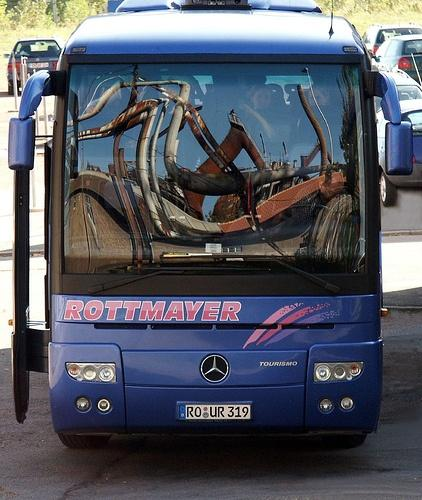
\includegraphics[width=0.11\textwidth]{image/improvement/2007_000663.jpg}
		\enspace\enspace %\hfill
		
\includegraphics[width=0.11\textwidth]{image/improvement/2007_000663.png}
		\enspace\enspace
		
\includegraphics[width=0.11\textwidth]{image/improvement/2007_000663_1.png}
		\enspace\enspace
		
\includegraphics[width=0.11\textwidth]{image/improvement/2007_000663_2.png}
		\enspace\enspace
		
\includegraphics[width=0.11\textwidth]{image/improvement/2007_000663_3.png}
		\enspace\enspace
		
\includegraphics[width=0.11\textwidth]{image/improvement/2007_000663_4.png}
		\enspace\enspace
		
\includegraphics[width=0.11\textwidth]{image/improvement/2007_000663_5.png}
		\enspace\enspace
		\caption[同一网络网格型长短记忆网络时序的增加对输出改善作用的可视化]{网格型长短记忆网络层数增加对输出改善作用的可视化}
		\label{fig:improvement}
	\end{figure}
}

\frame{
   \frametitle{与其它工作的定量对比}
\begin{table}[h] %voc table result
	\centering
		\resizebox{\textwidth}{!}{
		\begin{tabular}{c|*{20}{c}|c}
			\toprule
			Method & aero & bike & bird & boat & bottle & bus & car & cat & chair & cow & table & dog & horse & mbike & person & plant & shep & sofa & train & tv & mIoU.\\
			\midrule
			\midrule
			SDS\footnote{Simultaneous Detection and Segmentation, ECCV 2014}& 63.3 & 25.7 & 63.0 & 39.8 & 59.2 & 70.9 & 61.4 & 54.9 & 16.8 & 45.0 & 48.2 & 50.5 & 51.0 & 57.7 & 63.3 & 31.8 & 58.7 & 31.2 & 55.7 & 48.5 & 51.6 \\
			FCN-8s\footnote{Fully convolutional networks for semantic segmentation, CVPR 2015}  & 76.8 & 34.2 & 68.9 & 49.4 & 60.3 & 75.3 & 74.7 & 77.6 & 21.4 & 62.5 & 46.8 & 71.8 & 63.9 & 76.5 & 73.9 & 45.2 & 72.4 & 37.4 & 70.9 & 55.1 & 62.2\\
			TTI-zoomout-16\footnote{Feedforward semantic segmentation with zoom-out features, CVPR 2015} & \textbf{81.9} & 35.1 & \textbf{78.2} & \textbf{57.4} & 56.5 & 80.5 & 74.0 & 79.8 & 22.4 & 69.6 & 53.7 & 74.0 & \textbf{76.0} & 76.6 & 68.8 & 44.3 & 70.2 & 40.2 & 68.9 & 55.3 &	64.4 \\
			DeepLab-CRF\footnote{Semantic image segmentation with deep convolutional nets and fully connected crfs, ICLR 2015} & 78.4 & 33.1 & \textbf{78.2} & 55.6 & \textbf{65.3} & 81.3 & 75.5 & 78.6 & \textbf{25.3} & 69.2 & 52.7 & \textbf{75.2} & 69.0 & \textbf{79.1} & \textbf{77.6} & \textbf{54.7} & 78.3 & 45.1 & 73.3 & 56.2 & 66.4  \\
			\midrule
			CNN+\textbf{5}LSTM & 80.2 & \textbf{35.3} & 74.1 & 54.4 & 64.4 & \textbf{87.3} & \textbf{81.1} & \textbf{80.6} & 22.7 & \textbf{73.6} & \textbf{58.8} & 73.9 & 73.7 & 78.7 & 77.4 & 50.2 & \textbf{80.0} & \textbf{47.9} & \textbf{76.5} & \textbf{63.1} & \textbf{67.9} \\
			\bottomrule
		\end{tabular}}
		\caption[模型在VOC2012测试集上的结果]{模型在VOC2012测试集上的结果。}		
		\label{tab:voctest}
	\end{table}
	\vspace{-1em}
	\begin{block}{结论}
		\begin{itemize}
			\item[\dag]模型比其他方法有更高的精确度,验证了模型的有效性	
		\end{itemize}
	\end{block}
}
\frame{
   \frametitle{与其它工作的定性对比}
\begin{figure} % image examples & compare
	\begin{subfigure}{0.55\textwidth}
		\centering
		\makebox[0.18\textwidth]{\tiny Grid-5LSTM}
		\makebox[0.18\textwidth]{\tiny FCN-8s}
		\makebox[0.18\textwidth]{\tiny SDS}
		\makebox[0.18\textwidth]{\tiny 真值}
		\makebox[0.18\textwidth]{\tiny 图像} \\
		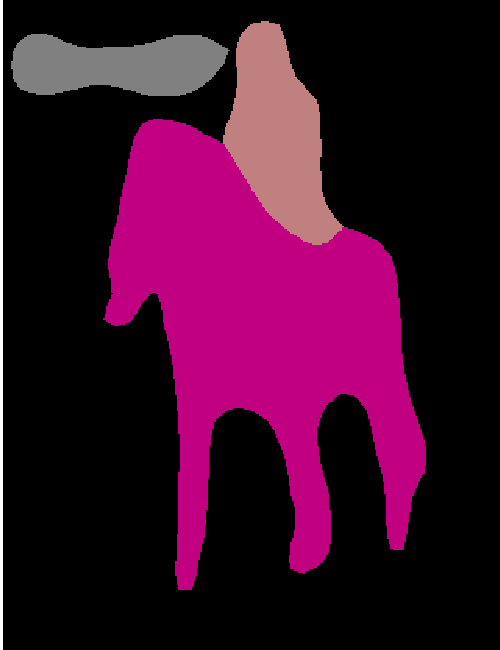
\includegraphics[width=0.18\textwidth]{image/result/compare/my_horse.pdf}
		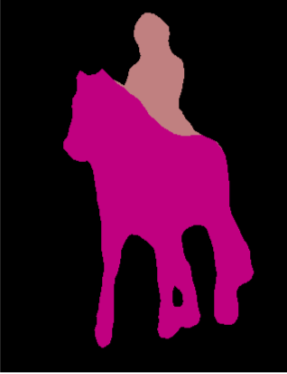
\includegraphics[width=0.18\textwidth]{image/result/compare/fcn_horse.png}
		
\includegraphics[width=0.18\textwidth]{image/result/compare/sds_horse.png}
		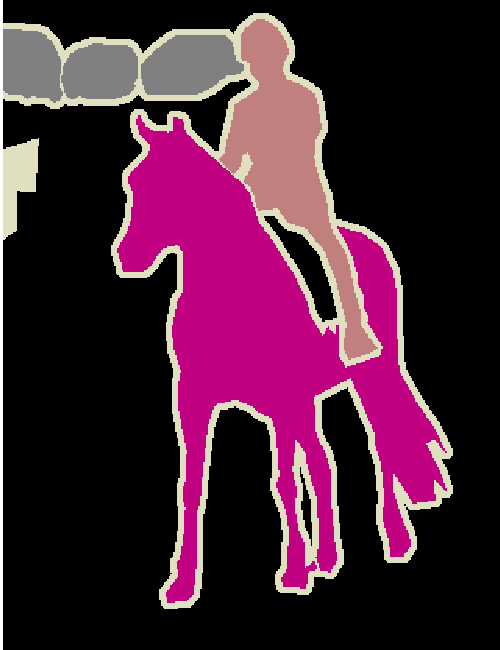
\includegraphics[width=0.18\textwidth]{image/result/compare/gt_horse.pdf}
		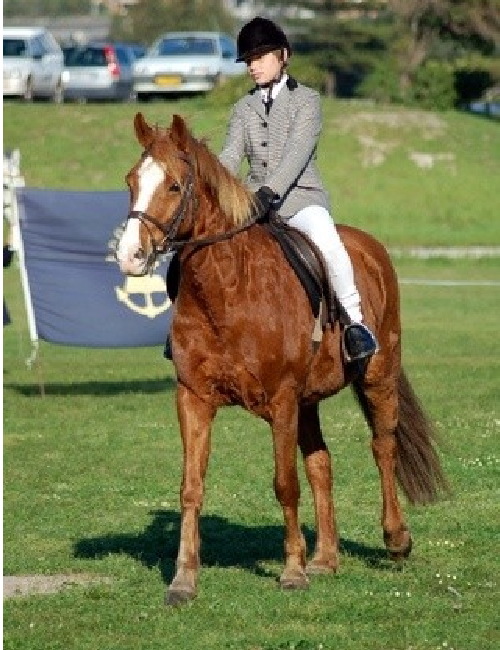
\includegraphics[width=0.18\textwidth]{image/result/compare/im_horse.pdf}
		\\
		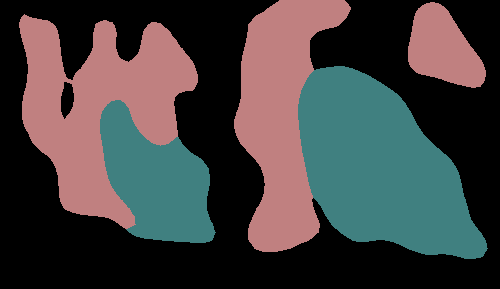
\includegraphics[width=0.18\textwidth]{image/result/compare/my_motor.png}
		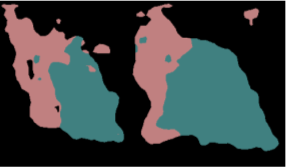
\includegraphics[width=0.18\textwidth]{image/result/compare/fcn_motor.png}
		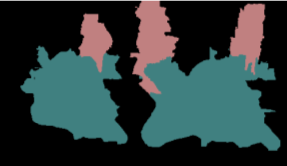
\includegraphics[width=0.18\textwidth]{image/result/compare/sds_motor.png}
		
\includegraphics[width=0.18\textwidth]{image/result/compare/2007_005173.png}
		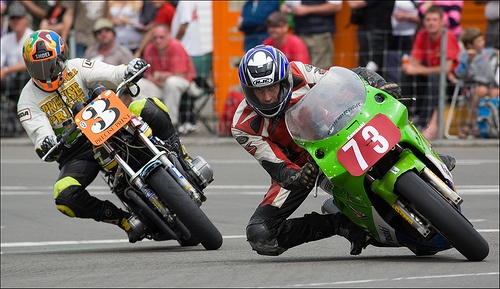
\includegraphics[width=0.18\textwidth]{image/result/compare/2007_005173.jpg}
		\\
		
\includegraphics[width=0.18\textwidth]{image/result/compare/my_sheep.pdf}
		
\includegraphics[width=0.18\textwidth]{image/result/compare/fcn_sheep.png}
		
\includegraphics[width=0.18\textwidth]{image/result/compare/sds_sheep.png}
		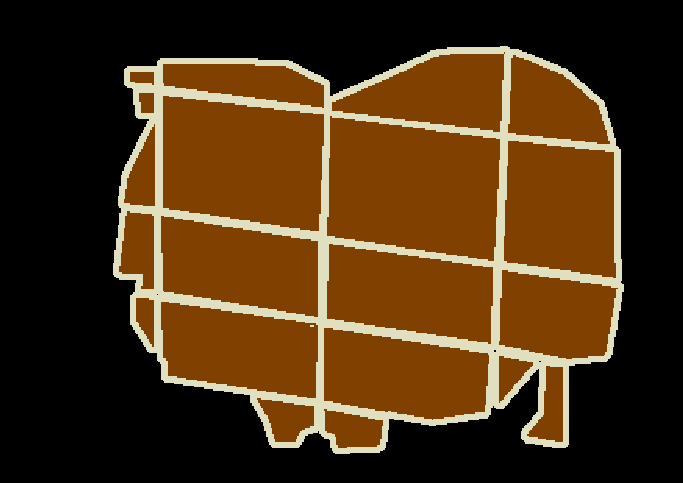
\includegraphics[width=0.18\textwidth]{image/result/compare/gt_sheep.pdf}
		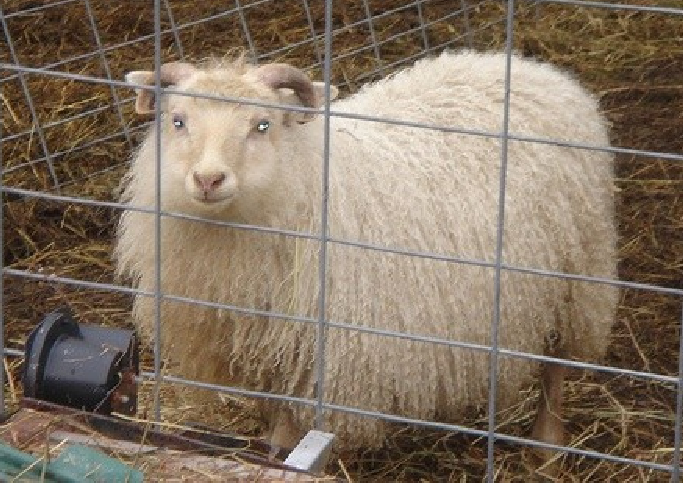
\includegraphics[width=0.18\textwidth]{image/result/compare/im_sheep.pdf}
		\\
		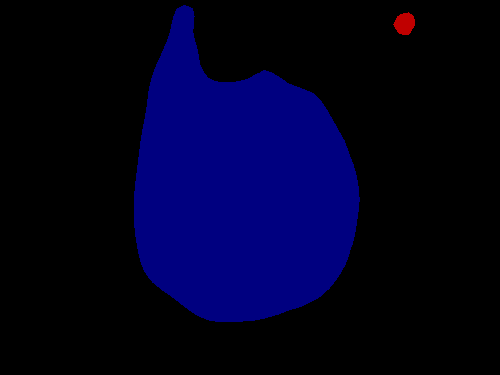
\includegraphics[width=0.18\textwidth]{image/result/compare/my_boat.png}
		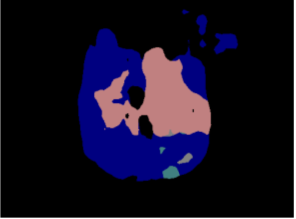
\includegraphics[width=0.18\textwidth]{image/result/compare/fcn_boat.png}
		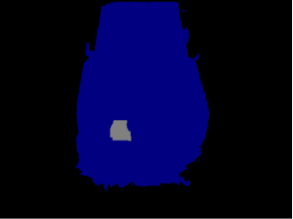
\includegraphics[width=0.18\textwidth]{image/result/compare/sds_boat.png}
		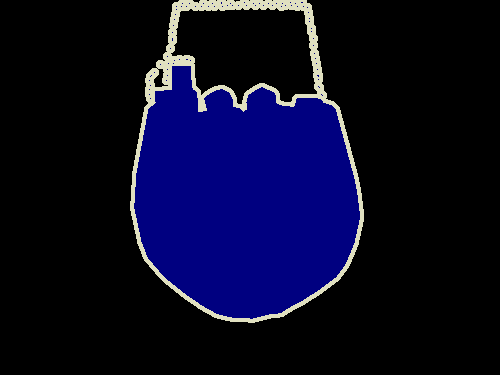
\includegraphics[width=0.18\textwidth]{image/result/compare/2007_004241.png}
		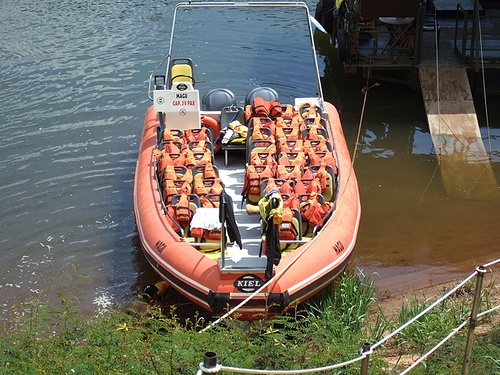
\includegraphics[width=0.18\textwidth]{image/result/compare/2007_004241.jpg}
		\caption{本文模型效果与其他工作的定性对比}
		\label{fig:compare1}
	\end{subfigure}
	\begin{subfigure}{0.4\textwidth}
		\centering

		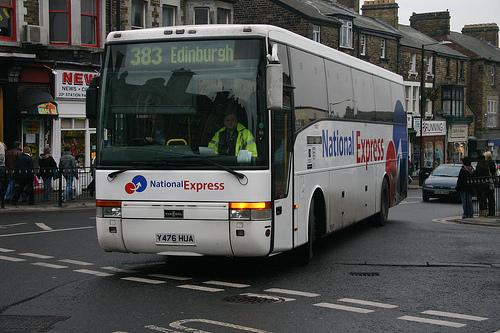
\includegraphics[width=0.25\textwidth]{image/result/compare/2010_005284.jpg}
		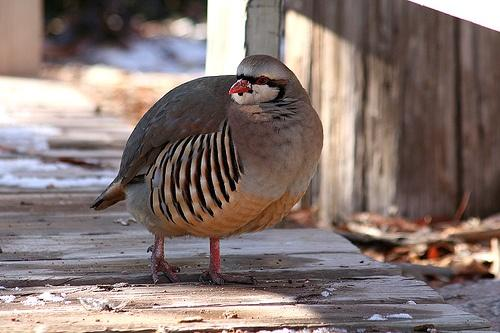
\includegraphics[width=0.25\textwidth]{image/result/compare/2007_003349.jpg}
		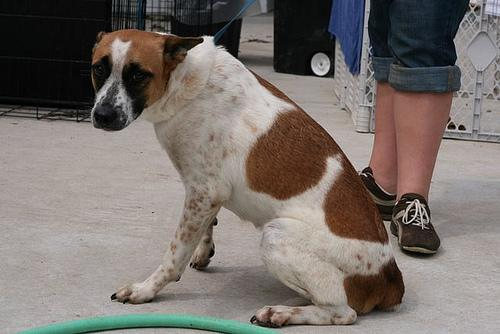
\includegraphics[width=0.25\textwidth]{image/result/compare/2009_004507.jpg} 
		\\
		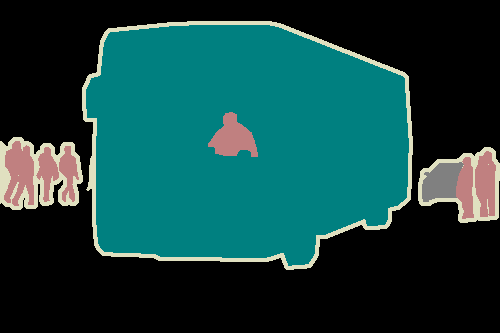
\includegraphics[width=0.25\textwidth]{image/result/compare/2010_005284.png}
		
\includegraphics[width=0.25\textwidth]{image/result/compare/2007_003349.png}
		
\includegraphics[width=0.25\textwidth]{image/result/compare/2009_004507.png} \\
		
\includegraphics[width=0.25\textwidth]{image/result/compare/zoom_bus.png}
		
\includegraphics[width=0.25\textwidth]{image/result/compare/zoom_bird.png}
		
\includegraphics[width=0.25\textwidth]{image/result/compare/zoom_dog.png} \\
		
\includegraphics[width=0.25\textwidth]{image/result/compare/deeplab_bus.png}
		
\includegraphics[width=0.25\textwidth]{image/result/compare/deeplab_bird.png}
		
\includegraphics[width=0.25\textwidth]{image/result/compare/deeplab_dog.png} \\
		
\includegraphics[width=0.25\textwidth]{image/result/compare/my_bus.png}
		
\includegraphics[width=0.25\textwidth]{image/result/compare/my_bird.png}
		\includegraphics[width=0.25\textwidth]{image/result/compare/my_dog.png} 
		\caption{\tiny 其中第一行为图像,第二行为真值,第三行为TTI-zoomout-16,第四行为DeepLab-CRF,第五行是Grid-5LSTM的结果}
		\label{fig:compare2}
	\end{subfigure}
	\caption{Grid-5LSTM与其它模型在VOC 2012验证集上的定性比较}
	\end{figure}
}

\frame{
   \frametitle{一些分割失败的例子}
	\begin{figure}[h]
		\centering
		\makebox[0.15\textwidth]{\footnotesize 图像}
		\makebox[0.15\textwidth]{\footnotesize 真值}
		\makebox[0.15\textwidth]{\tiny CNN+5LSTM}
		\quad
		\makebox[0.15\textwidth]{\footnotesize 图像} 
		\makebox[0.15\textwidth]{\footnotesize 真值}
		\makebox[0.15\textwidth]{\tiny CNN+5LSTM}\\
		\includegraphics[width=0.15\textwidth]{image/result/error/2008_000673.jpg}
		\includegraphics[width=0.15\textwidth]{image/result/error/2008_000673.png}
		\includegraphics[width=0.15\textwidth]{image/result/error/p_2008_000673.png} 
		\quad
		\includegraphics[width=0.15\textwidth]{image/result/error/2008_001580.jpg} 
		\includegraphics[width=0.15\textwidth]{image/result/error/2008_001580.png}
		\includegraphics[width=0.15\textwidth]{image/result/error/p_2008_001580.png} 
		\\
		\includegraphics[width=0.15\textwidth]{image/result/error/2007_002539.jpg}
		\includegraphics[width=0.15\textwidth]{image/result/error/2007_002539.png}
		\includegraphics[width=0.15\textwidth]{image/result/error/p_2007_002539.png}
		\quad
		\includegraphics[width=0.15\textwidth]{image/result/error/2007_008964.jpg}
		\includegraphics[width=0.15\textwidth]{image/result/error/2007_008964.png}
		\includegraphics[width=0.15\textwidth]{image/result/error/p_2007_008964.png}
		\\
		\includegraphics[width=0.15\textwidth]{image/result/error/2008_000763.jpg}
		\includegraphics[width=0.15\textwidth]{image/result/error/2008_000763.png}
		\includegraphics[width=0.15\textwidth]{image/result/error/p_2008_000763.png}
		\quad
		\includegraphics[width=0.15\textwidth]{image/result/error/2007_009088.jpg}
		\includegraphics[width=0.15\textwidth]{image/result/error/2007_009088.png}
		\includegraphics[width=0.15\textwidth]{image/result/error/p_2007_009088.png}
		\\
	\color[rgb]{0.9,0.9,0.9}\bfseries
	\resizebox{\textwidth}{!}{
	\begin{tabular}{*{7}{>{\centering\arraybackslash}p{0.111\textwidth}}}
		\hline
		\cellcolor[rgb]{0,0,0}  背景&\cellcolor[rgb]{0.5020,0,0} 飞机 &\cellcolor[rgb]{0,0.5020,0} 自行车 &\cellcolor[rgb]{0.5020,0.5020,0} 鸟 &\cellcolor[rgb]{0,0,0.5020} 船   &\cellcolor[rgb]{0.5020,0,0.5020} 瓶子 &\cellcolor[rgb]{0,0.5020,0.5020} 大巴
		\\
		\hline
		\cellcolor[rgb]{0.5020,0.5020,0.5020} 汽车 & \cellcolor[rgb]{0.2510,0,0} 猫 &\cellcolor[rgb]{0.7529,0,0} 椅子 &\cellcolor[rgb]{0.2510,0.5020,0} 牛 &\cellcolor[rgb]{0.7529,0.5020,0} 桌子 &\cellcolor[rgb]{0.2510,0,0.5020} 狗 &\cellcolor[rgb]{0.7529,0,0.5020} 马 \\
		\hline
		\cellcolor[rgb]{0.2510,0.5020,0.5020} 摩托车 &\cellcolor[rgb]{0.7529,0.5020,0.5020} 人   &\cellcolor[rgb]{0,0.2510,0} 盆栽   &\cellcolor[rgb]{0.5020,0.2510,0} 羊 &\cellcolor[rgb]{0,0.7529,0} 沙发 &\cellcolor[rgb]{0.5020,0.7529,0} 火车 &\cellcolor[rgb]{0,0.2510,0.5020} 电视 \\
		\hline
	\end{tabular}
	}
	\caption[一些模型分类错误的例子]{一些CNN+5LSTM分类错误的例子}
		\label{fig:error}
	\end{figure}
}

\subsection*{SIFT FLOW实验结果}
\frame{
   \frametitle{SIFT FLOW实验结果}
\begin{table}[h] %voc table result
	\centering
		\resizebox{0.8\textwidth}{!}{
		\begin{tabular}{*{4}{c}}
			\toprule
	 		Method & Pixel Acc. & Mean Acc. & Mean IU.\\
			\midrule
			Liu et al.\footnote{Sift flow: Dense correspondence across scenes and its applications, PAMI 2011}   & 76.7 & - & -\\
			Tighe et al.\footnote{Finding things: Image parsing with regions and per-exemplar detectors, CVPR 2013} & 78.6 & 39.2 & -\\
			FCN-16s\footnote{Fully convolutional networks for semantic segmentation, CVPR 2015} & 85.2 & \textbf{51.7} & 39.5\\
			Deeplab-LargeFOV\footnote{emantic image segmentation with deep convolutional nets and fully connected crfs, ICLR 2015}& 85.6 & 51.2 & 39.7\\
			\midrule
			Grid-5LSTM & \textbf{86.2} & 51.0 & \textbf{41.2}\\
			\bottomrule
		\end{tabular}
	}
		\caption[模型在SIFT FLOW上的结果]{模型在SIFT FLOW上的结果。Tighe等人的方法是用SVM+MRF,Deeplab-LargeFOV的结果是通过公开的源码实验得到的}		
		\label{tab:siftflow}
	\end{table}
}

\endinput
